% 8 Appendix D
\section{Appendix D}

\begin{guidance}
\centering
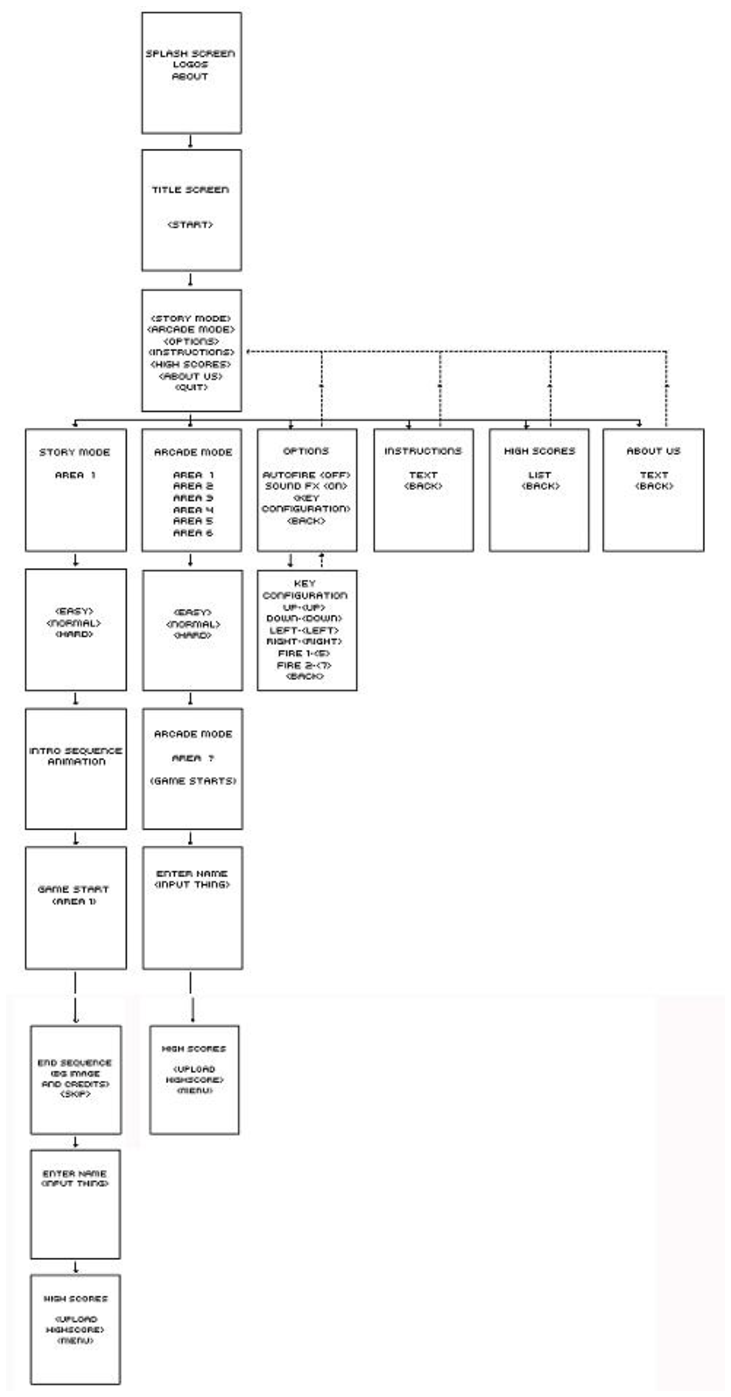
\includegraphics[width=\linewidth,height=0.82\textheight,keepaspectratio]{figures/appendix-d-game-architecture.pdf}
\end{guidance}
% Write your text below.

\subsection{Hold the Door -- Game Architecture Diagram}

The architecture diagram below outlines the screen hierarchy, UI navigation paths, and backend subsystem relationships governing the runtime lifecycle of \textbf{Hold the Door}.

\begin{figure}[htbp]
\centering
\begin{tikzpicture}[
  node distance=1.0cm and 1.2cm,
  screen/.style={rectangle, rounded corners=4pt, draw=black!80, fill=gddhead, thick, text width=2.6cm, align=center, inner sep=5pt, font=\small\bfseries},
  subscreen/.style={rectangle, draw=black!80, fill=white, thick, text width=2.4cm, align=center, inner sep=4pt, font=\footnotesize},
  system/.style={rectangle, rounded corners=2pt, draw=blue!70, fill=blue!5, thick, text width=2.5cm, align=center, inner sep=4pt, font=\footnotesize},
  arrow/.style={-{Stealth[scale=1.0]}, thick, draw=black!80}
]

% Screen Hierarchy
\node (title) [screen] {1.0 Splash \& Title Screen};
\node (menu) [screen, below=of title] {2.0 Main Menu Hub};
\node (settings) [subscreen, left=of menu] {2.1 Audio \& Video Settings};
\node (bestiary) [subscreen, right=of menu] {2.2 Bestiary \& Codex};
\node (levelselect) [screen, below=of menu] {3.0 Level Select Map};
\node (gameplay) [screen, below=of levelselect] {4.0 Combat Scene\\(Field \& Entities)};
\node (hud) [subscreen, left=of gameplay] {4.1 Real-Time HUD\\(HP, Gold, Wave, Speed)};
\node (radial) [subscreen, right=of gameplay] {4.2 Radial Build \& Upgrade Menu};
\node (pause) [subscreen, below left=of gameplay] {5.0 Pause Modal\\(Resume, Restart, Quit)};
\node (results) [screen, below right=of gameplay] {6.0 Stage Resolution\\(Victory / Defeat)};

% Screen Connections
\draw [arrow] (title) -- (menu);
\draw [arrow] (menu) -- (settings);
\draw [arrow] (menu) -- (bestiary);
\draw [arrow] (menu) -- (levelselect);
\draw [arrow] (levelselect) -- (gameplay);
\draw [arrow] (gameplay) -- (hud);
\draw [arrow] (gameplay) -- (radial);
\draw [arrow] (gameplay) -- (pause);
\draw [arrow] (gameplay) -- (results);
\draw [arrow] (results.south) -- ++(0,-0.4) -| (levelselect.east);

\end{tikzpicture}
\caption{Screen Hierarchy and UI Flow of \textbf{Hold the Door}}
\label{fig:screen-hierarchy}
\end{figure}

\subsection{Backend Software Subsystems}

The core Unity~6 execution layer is partitioned into decoupled singletons and ScriptableObjects communicating via C\# event delegates:

\begin{figure}[htbp]
\centering
\begin{tikzpicture}[
  node distance=0.8cm and 1.2cm,
  mgr/.style={rectangle, rounded corners=4pt, draw=gddnavy, fill=gddlabel, thick, text width=3.2cm, align=center, inner sep=6pt, font=\small\bfseries},
  data/.style={rectangle, draw=green!60!black, fill=green!10, thick, text width=3.0cm, align=center, inner sep=5pt, font=\footnotesize},
  entity/.style={rectangle, draw=red!70!black, fill=red!10, thick, text width=3.0cm, align=center, inner sep=5pt, font=\footnotesize},
  arrow/.style={-{Stealth[scale=1.0]}, thick, draw=black!80}
]

\node (gm) [mgr] {GameManager\\(Game State Controller)};
\node (econ) [mgr, left=of gm] {EconomyManager\\(Scrap, Transactions)};
\node (wave) [mgr, right=of gm] {WaveManager\\(Wave Sequencing)};
\node (door) [mgr, below=of gm] {FenceHealth\\(Fence HP, Breach Events)};

\node (waveso) [data, above=of wave] {WaveData (ScriptableObject)\\(Zombie Queues, Timings)};
\node (towerso) [data, above=of econ] {TowerData (ScriptableObject)\\(Single, Sniper, Shotgun)};

\node (pool) [mgr, below=of wave] {ObjectPoolManager\\(Zombies, Bullets)};
\node (towers) [entity, below=of econ] {Tower Instances\\(Targeting \& Firing)};
\node (enemies) [entity, below=of pool] {Zombie Instances\\(Left $\rightarrow$ Right Traversal)};

\draw [arrow] (gm) -- (econ);
\draw [arrow] (gm) -- (wave);
\draw [arrow] (gm) -- (door);
\draw [arrow] (waveso) -- (wave);
\draw [arrow] (towerso) -- (econ);
\draw [arrow] (wave) -- (pool);
\draw [arrow] (pool) -- (enemies);
\draw [arrow] (econ) -- (towers);
\draw [arrow] (enemies.west) -- (door.east);
\draw [arrow] (towers.east) -- node[above, font=\scriptsize] {Damage} (enemies.west);

\end{tikzpicture}
\caption{Decoupled Software Subsystem and Event Architecture}
\label{fig:software-architecture}
\end{figure}
